\documentclass{article}
\usepackage{CJKutf8}
\usepackage{graphicx}
\usepackage{math_blog}
\usepackage{amsmath}
\usepackage{appendix}
\usepackage[normalem]{ulem}
\usepackage[thicklines]{cancel}
\usepackage{tikz}
\usetikzlibrary{positioning,arrows.meta}
\usepackage{pgfplots}

% Defensive: resolve possible \proof / theorem-env conflicts with math_blog
\makeatletter
\@ifundefined{proof}{}{\let\proof\@undefined \let\endproof\@undefined}
\@ifundefined{theorem}{\newtheorem{theorem}{Theorem}[section]}{}
\@ifundefined{lemma}{\newtheorem{lemma}[theorem]{Lemma}}{}
\@ifundefined{definition}{\newtheorem{definition}[theorem]{Definition}}{}
\makeatother
\newenvironment{proof}[1][Proof]{%
  \par\smallskip\noindent\textit{\textbf{#1.}}\quad\ignorespaces
}{%
  \hfill$\square$\par\smallskip
}

\title{[SDE III] Existence, Uniqueness, and the SDE-PDE Bridge}
\author{Anqiao Ouyang, Xuecheng Liu}
\date{May 26, 2026}

\newcommand{\Title}{Existence, Uniqueness, and the SDE--PDE Bridge}

\newcommand{\Column}{Stochastic Differential Equations III}
\newcommand{\Author}{Anqiao Ouyang}

\begin{document}
\begin{CJK*}{UTF8}{gbsn}

\maketitle

\section{Introduction}

In the previous two articles we built up the basic machinery: Brownian motion as a continuous, nowhere-differentiable driving process, the It\^o integral as the right way to integrate against it, and the It\^o formula as the chain rule for stochastic dynamics. We also discussed numerical schemes (Euler--Maruyama, Milstein), and along the way we used several results: existence of solutions, the Markov property, the parabolic operator $\partial_t+\mathcal L$ acting on conditional expectations, that were stated but not proved in full.

This article fills in those gaps and pushes one step further. We address three intertwined questions:
\begin{enumerate}
    \item Under what conditions does an SDE
    \[
      \mathrm{d}X_t=a(t,X_t)\,\mathrm{d}t+b(t,X_t)\,\mathrm{d}B_t,\qquad X_0=x_0
    \]
    have a solution, and is that solution unique? What does ``solution'' even mean here?
    \item Once a solution exists, what is its probabilistic structure? In particular, why is it Markov, and what is the right object to read off the law of $X_t$ from?
    \item How does the SDE talk to deterministic PDEs? The conditional expectation $u(t,x)=\mathbb{E}[f(X_T)\mid X_t=x]$ already appeared as a magic ingredient in the weak-convergence proof of the EM scheme; here we explain why it solves a parabolic equation, derive the Fokker--Planck equation for the marginal density, and connect everything to the Feynman--Kac formula and Girsanov's theorem.
\end{enumerate}

The thread tying these together is the \textbf{infinitesimal generator} $\mathcal L=a\partial_x+\tfrac12 b^2\partial_{xx}$. It encodes the SDE; it determines the transition semigroup; it is the spatial operator in both Kolmogorov equations; and Feynman--Kac is essentially the statement that $\partial_t+\mathcal L$ has a stochastic representation.

\section{Existence and Uniqueness}

\subsection{Strong vs.\ Weak Solutions}

Two notions of solution coexist in SDE theory, and they answer different questions.

\begin{definition}[Strong solution]
Fix a probability space $(\Omega,\mathcal{F},\mathbb{P})$, a Brownian motion $B$, and the filtration $\{\mathcal{F}_t\}$ generated by $B$ (augmented to satisfy the usual conditions). A \textbf{strong solution} to
\begin{equation}\label{eq:sde}
    \mathrm{d}X_t=a(t,X_t)\,\mathrm{d}t+b(t,X_t)\,\mathrm{d}B_t,\qquad X_0=\xi,
\end{equation}
is an $\{\mathcal{F}_t\}$-adapted process $X$ with continuous sample paths such that
\[
  X_t=\xi+\int_0^t a(s,X_s)\,\mathrm{d}s+\int_0^t b(s,X_s)\,\mathrm{d}B_s,\qquad \forall t\in[0,T]\ \text{a.s.}
\]
\end{definition}

In words: the driving Brownian motion is fixed up front, and the solution is a measurable functional of its path. This is the right notion when you want to simulate, since the EM scheme builds $\bar{X}^\delta$ pathwise from a single Brownian sample.

\begin{definition}[Weak solution]
A \textbf{weak solution} is a tuple $(\Omega,\mathcal{F},\mathbb{P},\{\mathcal{F}_t\},B,X)$ such that $B$ is an $\{\mathcal{F}_t\}$-Brownian motion on this space and $X$ satisfies the integral equation above. Here the Brownian motion and the probability space are part of the answer, not the question.
\end{definition}

Weak solutions are sufficient for any question about the \emph{law} of $X$ (distributional properties, moments, transition probabilities), since one is free to choose a convenient space. Strong solutions are needed when the relationship between $X$ and a specific $B$ matters (simulation, filtering, pathwise control).

A strong solution is automatically a weak solution. The converse can fail: there are SDEs (Tanaka's example $\mathrm{d}X_t=\operatorname{sgn}(X_t)\,\mathrm{d}B_t$ is the canonical one) which admit a weak solution but no strong solution. Throughout this article we focus on strong solutions, since the standard Lipschitz framework delivers them directly.

\subsection{The Picard--Lindel\"of Argument, Stochastically}

In the deterministic case, existence and uniqueness for $\dot x=f(t,x)$ with $f$ Lipschitz in $x$ is proved by Picard iteration: define $x^{(n+1)}_t=x_0+\int_0^t f(s,x^{(n)}_s)\,\mathrm{d}s$ and show $\{x^{(n)}\}$ is Cauchy in $C([0,T])$. The stochastic version uses the same skeleton, with $L^2(\Omega)$ replacing pointwise estimates and the It\^o isometry doing the heavy lifting on the diffusion term.

Let us write down the assumptions in one place. These are the same Conditions 1--4 used implicitly in [II] for the convergence of the EM scheme.

\begin{itemize}
    \item \textbf{(L) Lipschitz:} there exists $L>0$ with
    $|a(t,x)-a(t,y)|+|b(t,x)-b(t,y)|\le L|x-y|$ for all $t\in[0,T]$, $x,y\in\mathbb{R}$.
    \item \textbf{(G) Linear growth:} there exists $C>0$ with
    $|a(t,x)|^2+|b(t,x)|^2\le C(1+|x|^2)$.
    \item \textbf{(I) Initial data:} $\xi$ is $\mathcal{F}_0$-measurable with $\mathbb{E}|\xi|^2<\infty$.
\end{itemize}

\begin{theorem}[Existence and uniqueness of strong solutions]\label{thm:exuniq}
Under (L), (G), (I), the SDE \eqref{eq:sde} admits a unique strong solution $X\in L^2_T(\Omega)$ with continuous sample paths. Moreover,
\[
  \mathbb{E}\!\left[\sup_{0\le t\le T}|X_t|^2\right]\le K\,(1+\mathbb{E}|\xi|^2)
\]
for a constant $K$ depending only on $L,C,T$.
\end{theorem}

The proof splits into three estimates: an a priori moment bound, the Cauchy property of the Picard sequence, and pathwise uniqueness. We sketch the structure here and defer details to Appendix~\ref{app:exuniq}.

\paragraph{Step 1: A priori bound.} Define $\Phi:L^2_T(\Omega)\to L^2_T(\Omega)$ by
\[
  (\Phi X)_t=\xi+\int_0^t a(s,X_s)\,\mathrm{d}s+\int_0^t b(s,X_s)\,\mathrm{d}B_s.
\]
We claim $\Phi$ maps $L^2_T$ into itself. By Cauchy--Schwarz on the drift integral and the It\^o isometry on the diffusion integral,
\[
  \mathbb{E}|(\Phi X)_t|^2\le 3\mathbb{E}|\xi|^2+3T\,\mathbb{E}\!\int_0^t|a(s,X_s)|^2\,\mathrm{d}s+3\,\mathbb{E}\!\int_0^t|b(s,X_s)|^2\,\mathrm{d}s.
\]
Plugging in (G),
\[
  \mathbb{E}|(\Phi X)_t|^2\le 3\mathbb{E}|\xi|^2+3(T+1)C\!\int_0^t\!\bigl(1+\mathbb{E}|X_s|^2\bigr)\,\mathrm{d}s,
\]
which is finite for $X\in L^2_T$.

\paragraph{Step 2: Picard iteration.} Set $X^{(0)}_t\equiv\xi$ and $X^{(n+1)}=\Phi X^{(n)}$. A standard computation using the Lipschitz bound (L) yields
\[
  \mathbb{E}\!\left[\sup_{s\le t}|X^{(n+1)}_s-X^{(n)}_s|^2\right]\le K_1\!\int_0^t\mathbb{E}\!\left[\sup_{r\le s}|X^{(n)}_r-X^{(n-1)}_r|^2\right]\mathrm{d}s.
\]
The Doob $L^2$ maximal inequality is what lets us pull the $\sup$ inside the expectation on the diffusion piece. Iterating $n$ times,
\[
  \mathbb{E}\!\left[\sup_{s\le T}|X^{(n+1)}_s-X^{(n)}_s|^2\right]\le \frac{(K_1 T)^n}{n!}\,M_0,
\]
where $M_0=\mathbb{E}\sup_{s\le T}|X^{(1)}_s-X^{(0)}_s|^2<\infty$. The series $\sum_n \sqrt{(K_1T)^n/n!}$ converges, so $\{X^{(n)}\}$ is Cauchy in the Banach space $\mathcal{S}^2_T$ of adapted continuous processes with norm $\|X\|_{\mathcal{S}^2}=\bigl(\mathbb{E}\sup_{s\le T}|X_s|^2\bigr)^{1/2}$. Its limit $X$ is a strong solution.

\paragraph{Step 3: Uniqueness.} Suppose $X,Y$ both solve \eqref{eq:sde}. Mimicking Step 2 on $X-Y$ and applying Gronwall (Appendix~\ref{app:gronwall}) gives $\mathbb{E}\sup_{s\le T}|X_s-Y_s|^2=0$, hence $X=Y$ indistinguishably.

\medskip

A few remarks are in order.

\begin{itemize}
    \item The Lipschitz assumption can be substantially weakened. \textbf{Yamada--Watanabe} shows pathwise uniqueness for 1D SDEs when $b$ is only $\rho$-H\"older with $\rho\ge 1/2$ and a modulus condition $\int_0^\varepsilon \rho^{-2}=\infty$. The square root in the CIR model $\mathrm{d}X_t=\kappa(\theta-X_t)\,\mathrm{d}t+\sigma\sqrt{X_t}\,\mathrm{d}B_t$ lives on this boundary. it is \emph{not} Lipschitz, but Yamada--Watanabe still gives uniqueness.
    \item Without linear growth, solutions can blow up in finite time. The \textbf{explosion} time
    $\tau_\infty=\lim_{n\to\infty}\inf\{t:|X_t|\ge n\}$
    may be finite a.s.\ (e.g.\ $\mathrm{d}X_t=X_t^2\,\mathrm{d}t$ with $X_0>0$). Standard practice is to localize: solve up to $\tau_n$, then check $\mathbb{P}(\tau_\infty>T)=1$.
    \item The bound (G) is essentially sharp for moment control. Without it, even when a solution exists pathwise, $\mathbb{E}|X_t|^2$ may be infinite.
\end{itemize}

\section{The Markov Property and the Generator}

\subsection{Markovianity}

The deterministic ODE $\dot x=f(t,x)$ has a trivial flow property: the trajectory after time $s$ depends only on $x_s$, not on how we got there. The same is true for solutions to time-homogeneous SDEs, but now ``depends only on $X_s$'' must be promoted to a statement about \emph{conditional distributions} rather than functional values.

\begin{theorem}[Markov property]\label{thm:markov}
Let $X$ be the strong solution of \eqref{eq:sde} with coefficients $a(x),b(x)$ time-homogeneous and Lipschitz. Then for any bounded measurable $f:\mathbb{R}\to\mathbb{R}$ and any $0\le s\le t\le T$,
\[
  \mathbb{E}\bigl[f(X_t)\mid \mathcal{F}_s\bigr]=\mathbb{E}\bigl[f(X_t)\mid X_s\bigr]\qquad\text{a.s.}
\]
\end{theorem}

\begin{proof}[Sketch]
The key observation is that the SDE solution starting at time $s$ from value $X_s$ depends only on the Brownian increments $B_u-B_s$ for $u\ge s$, which are independent of $\mathcal{F}_s$. Writing $X_t=\Psi(s,t,X_s,(B_u-B_s)_{s\le u\le t})$ where $\Psi$ is the deterministic functional that maps the initial condition and the driving path to the solution (this is well-defined by the existence/uniqueness theorem and the path-by-path nature of Picard iteration), we have $\mathbb{E}[f(X_t)\mid\mathcal{F}_s]=\Phi(X_s)$ where
\[
  \Phi(x)=\mathbb{E}\bigl[f(\Psi(s,t,x,(B_u-B_s)_{s\le u\le t}))\bigr].
\]
The right side is a deterministic function of $x$, hence $\sigma(X_s)$-measurable, and equals $\mathbb{E}[f(X_t)\mid X_s]$ by the tower property.
\end{proof}

Time-inhomogeneous SDEs are still Markov, but the transition probability depends on both endpoints $(s,t)$ rather than just the difference $t-s$.

\subsection{The Semigroup of Transition Operators}

The Markov property invites a functional-analytic reformulation. For time-homogeneous coefficients, define the operator $P_t:B_b(\mathbb{R})\to B_b(\mathbb{R})$ (bounded measurable functions) by
\[
  P_t f(x)=\mathbb{E}_x[f(X_t)]:=\mathbb{E}\bigl[f(X_t)\mid X_0=x\bigr].
\]
By the Markov property and time-homogeneity, $\{P_t\}_{t\ge 0}$ is a \textbf{semigroup}:
\[
  P_{t+s}f(x)=\mathbb{E}_x[f(X_{t+s})]=\mathbb{E}_x[\mathbb{E}[f(X_{t+s})\mid\mathcal{F}_s]]=\mathbb{E}_x[P_t f(X_s)]=P_s(P_t f)(x).
\]
The interpretation: $P_t$ propagates the observable $f$ backward in time by an amount $t$, in the sense that $P_t f(x)$ tells you the expected payoff of $f(X_t)$ from initial position $x$.

\subsection{The Infinitesimal Generator}

The semigroup is naturally analyzed via its infinitesimal generator. Heuristically,
\[
  \mathcal{L}f(x)=\lim_{t\downarrow 0}\frac{P_t f(x)-f(x)}{t}.
\]
For an SDE with smooth coefficients, the generator coincides with the parabolic operator we have been writing all along.

\begin{theorem}[Generator of an It\^o diffusion]\label{thm:generator}
Let $X$ solve $\mathrm{d}X_t=a(X_t)\,\mathrm{d}t+b(X_t)\,\mathrm{d}B_t$ with $a,b$ Lipschitz, and let $f\in C^2_b(\mathbb{R})$. Then
\[
  \mathcal{L}f(x)=a(x)f'(x)+\tfrac{1}{2}b^2(x)f''(x),
\]
and the limit holds uniformly in $x$.
\end{theorem}

\begin{proof}
By It\^o's formula applied to $f(X_t)$ with $X_0=x$,
\[
  f(X_t)-f(x)=\int_0^t \bigl(a f'+\tfrac{1}{2}b^2 f''\bigr)(X_s)\,\mathrm{d}s+\int_0^t b(X_s)f'(X_s)\,\mathrm{d}B_s.
\]
Taking expectations the stochastic integral vanishes (its integrand is in $L^2_T$ since $f',b$ are bounded on the range of $X_s$ over $[0,t]$, by linear growth). Dividing by $t$,
\[
  \frac{P_tf(x)-f(x)}{t}=\frac{1}{t}\mathbb{E}_x\!\int_0^t\mathcal{L}f(X_s)\,\mathrm{d}s\xrightarrow{t\downarrow 0}\mathcal{L}f(x)
\]
by continuity of $\mathcal{L}f(X_s)$ in $s$ (since $X$ is continuous and $\mathcal{L}f$ is continuous and bounded).
\end{proof}

\begin{figure}[h]
\centering
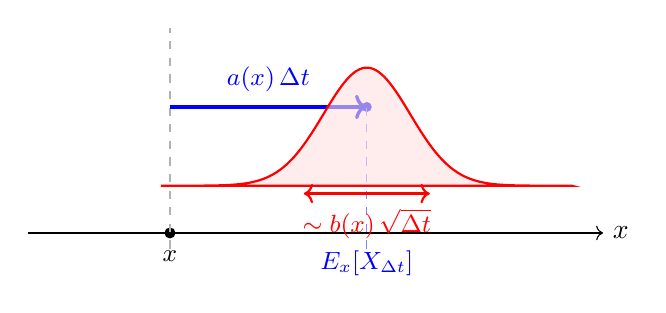
\begin{tikzpicture}[scale=1.0]
\draw[->] (-0.3,0) -- (7,0) node[right] {$x$};
\fill (1.5,0) circle (2pt) node[below=3pt] {\small$x$};
\draw[dashed, gray!60] (1.5,-0.2) -- (1.5,2.6);

\draw[->, blue, very thick] (1.5,1.6) -- (4,1.6);
\node[blue, above=2pt] at (2.75,1.6) {\small $a(x)\,\Delta t$};
\fill[blue] (4,1.6) circle (1.8pt);
\draw[dashed, blue!50] (4,-0.2) -- (4,1.6);
\node[blue, below=3pt] at (4,0) {\small $\mathbb{E}_x[X_{\Delta t}]$};

\draw[red, thick, fill=red!12, fill opacity=0.6]
  plot[domain=1.4:6.6, samples=60, smooth] (\x, {0.6 + 1.5*exp(-(\x-4)^2/(2*0.55^2))})
  -- (6.6,0.6) -- (1.4,0.6) -- cycle;
\draw[<->, red, thick] (3.2,0.5) -- (4.8,0.5);
\node[red, below=2pt] at (4,0.5) {\small $\sim b(x)\,\sqrt{\Delta t}$};
\end{tikzpicture}
\caption{The generator $\mathcal{L}=a\partial_x+\tfrac{1}{2}b^2\partial_{xx}^2$ visualized locally. Starting at $x$, over a small time $\Delta t$ the drift contributes a deterministic displacement of order $a(x)\Delta t$ (blue arrow), while the diffusion adds a Gaussian fluctuation of order $b(x)\sqrt{\Delta t}$ (red cloud). For small $\Delta t$, $\sqrt{\Delta t}\gg\Delta t$, so the diffusion dominates, which is why $\mathcal L$ must contain a second-order term, with coefficient $\tfrac12 b^2$ to balance the $\Delta t$ scaling of the variance.}
\label{fig:generator}
\end{figure}

Note the asymmetry: the drift contributes a first-order term, the diffusion a second-order term. This is a direct consequence of the It\^o calculus identity $(\mathrm{d}B_t)^2=\mathrm{d}t$, diffusion ``moves twice as fast'' as drift on the infinitesimal scale, which is what produces the $\tfrac{1}{2}b^2$ factor.

\section{Kolmogorov's Backward and Forward Equations}

The generator $\mathcal{L}$ governs two PDEs, dual to one another, that completely determine the law of $X$.

\subsection{Backward Equation}

Fix a terminal time $T$ and a payoff $f\in C_b(\mathbb{R})$. Define
\[
  u(t,x)=\mathbb{E}\bigl[f(X_T)\mid X_t=x\bigr]=P_{T-t}f(x).
\]
This is the conditional expectation that already appeared in [II] inside the weak-convergence argument for the EM scheme. The backward equation says it solves a deterministic PDE.

\begin{theorem}[Kolmogorov backward equation]\label{thm:backward}
Assume $a,b$ are Lipschitz with all derivatives bounded, and $f\in C^2_P$ (polynomial growth). Then $u(t,x)=\mathbb{E}_{t,x}[f(X_T)]$ is in $C^{1,2}([0,T)\times\mathbb{R})$ and satisfies
\[
  \begin{cases}
    \partial_t u(t,x)+\mathcal{L}u(t,x)=0,& (t,x)\in[0,T)\times\mathbb{R},\\
    u(T,x)=f(x).
  \end{cases}
\]
\end{theorem}

\begin{proof}[Sketch]
Apply It\^o's formula to $u(s,X_s)$ between $s=t$ and $s=T$, conditional on $X_t=x$:
\[
  u(T,X_T)-u(t,x)=\int_t^T(\partial_s u+\mathcal{L}u)(s,X_s)\,\mathrm{d}s+\int_t^T b(X_s)\partial_x u(s,X_s)\,\mathrm{d}B_s.
\]
Taking expectations conditional on $X_t=x$, the diffusion term has zero mean (by the moment estimate that follows from polynomial growth of $\partial_x u$). The left side is $\mathbb{E}_{t,x}[f(X_T)]-u(t,x)=0$ by definition of $u$. Hence
\[
  \mathbb{E}_{t,x}\!\int_t^T(\partial_s u+\mathcal{L}u)(s,X_s)\,\mathrm{d}s=0
\]
for all $(t,x)$. Differentiating in $t$ at $s=t$ and using continuity yields $(\partial_t u+\mathcal{L}u)(t,x)=0$. The boundary condition $u(T,x)=f(x)$ is immediate.

The regularity claim $u\in C^{1,2}$ is the hard part, and is why we assumed bounded derivatives of $a,b$. It can be proved by either differentiating the SDE in $x$ (the \textbf{stochastic flow} approach) or by appealing to the standard theory of uniformly parabolic PDEs.
\end{proof}

The name ``backward'' refers to the fact that the PDE evolves in the time variable that runs backward from the terminal data $T$: as $t$ decreases from $T$, we accumulate more information about $f(X_T)$.

\subsection{Forward Equation (Fokker--Planck)}

If we instead fix the initial law $X_0\sim\rho_0$ and ask for the density $\rho(t,x)$ of $X_t$, we get the dual equation.

\begin{theorem}[Fokker--Planck equation]\label{thm:fpe}
Suppose $X_t$ has a smooth density $\rho(t,x)$ for each $t>0$ (which holds e.g.\ when $b^2$ is uniformly elliptic, $b^2\ge\beta>0$). Then $\rho$ satisfies
\[
  \partial_t\rho(t,x)=-\partial_x\bigl(a(x)\rho(t,x)\bigr)+\tfrac{1}{2}\,\partial_{xx}^2\bigl(b^2(x)\rho(t,x)\bigr)=\mathcal{L}^*\rho,
\]
with initial condition $\rho(0,\cdot)=\rho_0$.
\end{theorem}

\begin{proof}[Sketch]
Pick any test function $\varphi\in C_c^\infty(\mathbb{R})$. By It\^o,
\[
  \mathbb{E}\varphi(X_t)-\mathbb{E}\varphi(X_0)=\mathbb{E}\!\int_0^t\mathcal{L}\varphi(X_s)\,\mathrm{d}s.
\]
Differentiating in $t$:
\[
  \frac{\mathrm{d}}{\mathrm{d}t}\!\int\varphi(x)\rho(t,x)\,\mathrm{d}x=\int\mathcal{L}\varphi(x)\rho(t,x)\,\mathrm{d}x=\int\varphi(x)\,\mathcal{L}^*\rho(t,x)\,\mathrm{d}x,
\]
where we integrated by parts to define the formal adjoint $\mathcal{L}^*\rho=-\partial_x(a\rho)+\tfrac{1}{2}\partial_{xx}^2(b^2\rho)$. Since $\varphi$ is arbitrary, $\partial_t\rho=\mathcal{L}^*\rho$ in the distributional sense; smoothness of $\rho$ then upgrades this to a classical PDE.
\end{proof}

\begin{figure}[h]
\centering
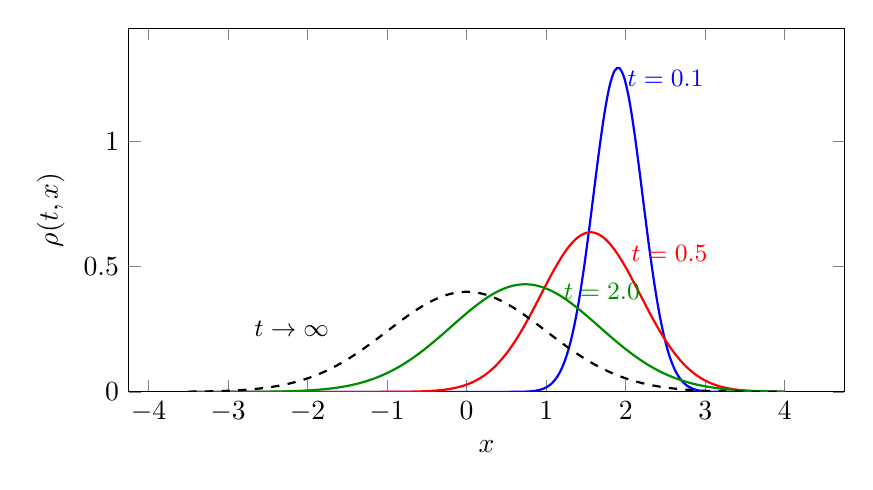
\begin{tikzpicture}
\begin{axis}[
    width=0.88\textwidth, height=6.2cm,
    xlabel={$x$}, ylabel={$\rho(t,x)$},
    domain=-3.5:4, samples=120,
    no markers, smooth,
    ymin=0, ymax=1.45,
]
\addplot[blue, thick] {1/sqrt(2*pi*0.0952) * exp(-(x-1.903)^2/(2*0.0952))};
\addplot[red, thick] {1/sqrt(2*pi*0.393) * exp(-(x-1.558)^2/(2*0.393))};
\addplot[green!55!black, thick] {1/sqrt(2*pi*0.865) * exp(-(x-0.736)^2/(2*0.865))};
\addplot[black, dashed, thick] {1/sqrt(2*pi) * exp(-x^2/2)};
\node[blue]    at (axis cs:2.5,1.25) {\small $t=0.1$};
\node[red]     at (axis cs:2.55,0.55) {\small $t=0.5$};
\node[green!55!black] at (axis cs:1.7,0.4) {\small $t=2.0$};
\node          at (axis cs:-2.2,0.25) {\small $t\to\infty$};
\end{axis}
\end{tikzpicture}
\caption{Solution of the Fokker--Planck equation for the OU process $\mathrm{d}X_t=-\tfrac{1}{2}X_t\,\mathrm{d}t+\mathrm{d}B_t$ started from $X_0=2$ (Dirac mass). The density translates leftward toward the mean $\mu=0$ at rate $\theta$ and broadens at rate $\sigma$ until it relaxes to the stationary $\mathcal{N}(0,1)$ (dashed). Both motions are encoded in $\mathcal{L}^*$: the $-\partial_x(a\rho)$ term shifts mass, the $\tfrac12\partial^2_{xx}(b^2\rho)$ term spreads it.}
\label{fig:fpe}
\end{figure}

\subsection{Backward vs.\ Forward at a Glance}

It is worth seeing the two equations side by side:
\[
  \begin{array}{l|ll}
  & \text{Backward (Kolmogorov)} & \text{Forward (Fokker--Planck)}\\
  \hline
  \text{Unknown} & u(t,x)=\mathbb{E}_{t,x}[f(X_T)] & \rho(t,x)=\text{density of }X_t\\
  \text{PDE} & \partial_t u+\mathcal{L}u=0 & \partial_t\rho=\mathcal{L}^*\rho\\
  \text{Data} & \text{terminal: }u(T,\cdot)=f & \text{initial: }\rho(0,\cdot)=\rho_0\\
  \text{Variable in }\mathcal{L} & \text{starting point }x & \text{current point }x\\
  \text{Solves in time} & \text{backward from }T & \text{forward from }0
  \end{array}
\]

The dichotomy is the standard one between the Schr\"odinger and Heisenberg pictures, between covariant and contravariant evolution: $u$ evolves observables, $\rho$ evolves states, and the two operators $\mathcal{L},\mathcal{L}^*$ are dual under the pairing $\langle u,\rho\rangle=\int u\rho\,\mathrm{d}x$.

\subsection{Stationary Distributions}

A \textbf{stationary} (or \textbf{invariant}) distribution $\pi$ satisfies $\mathcal{L}^*\pi=0$. If $X_0\sim\pi$, then $X_t\sim\pi$ for all $t$.

For 1D SDEs, the stationary density (when it exists and is integrable) can be written explicitly. From $\mathcal{L}^*\pi=-\partial_x(a\pi)+\tfrac12\partial_{xx}^2(b^2\pi)=0$, integrate once to get a first-order ODE
\[
  \tfrac{1}{2}\,(b^2\pi)'-a\pi=\text{const},
\]
and for stationary densities decaying at infinity the constant is zero. This gives
\[
  \pi(x)\propto\frac{1}{b^2(x)}\exp\!\left(\int^x \frac{2a(y)}{b^2(y)}\,\mathrm{d}y\right).
\]

\paragraph{Example: OU process.} For $\mathrm{d}X_t=\theta(\mu-X_t)\,\mathrm{d}t+\sigma\,\mathrm{d}B_t$ the formula gives
\[
  \pi(x)\propto\exp\!\left(-\frac{\theta(x-\mu)^2}{\sigma^2}\right),
\]
which is $\mathcal{N}(\mu,\sigma^2/(2\theta))$, exactly matching the long-time limit derived in [II] from the explicit solution.

\begin{figure}[h]
\centering
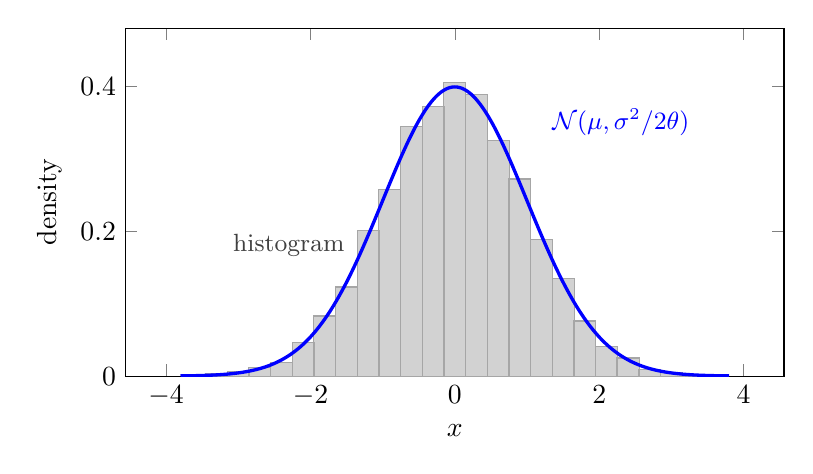
\begin{tikzpicture}
\begin{axis}[
    width=0.82\textwidth, height=6cm,
    xlabel={$x$}, ylabel={density},
    domain=-3.8:3.8, samples=120,
    ymin=0, ymax=0.48,
    no markers,
]
\addplot[ybar, bar width=0.28cm, fill=gray!35, draw=gray!70] coordinates {
    (-3.3, 0.003) (-3.0, 0.006) (-2.7, 0.012) (-2.4, 0.019) (-2.1, 0.047)
    (-1.8, 0.083) (-1.5, 0.123) (-1.2, 0.201) (-0.9, 0.258) (-0.6, 0.345)
    (-0.3, 0.372) (0.0, 0.405) (0.3, 0.388) (0.6, 0.325) (0.9, 0.272)
    (1.2, 0.189) (1.5, 0.135) (1.8, 0.076) (2.1, 0.041) (2.4, 0.025)
    (2.7, 0.009) (3.0, 0.005) (3.3, 0.002)
};
\addplot[blue, very thick, smooth] {1/sqrt(2*pi) * exp(-x^2/2)};
\node[blue] at (axis cs:2.3,0.35) {\small $\mathcal{N}(\mu,\sigma^2/2\theta)$};
\node[gray!50!black] at (axis cs:-2.3,0.18) {\small histogram};
\end{axis}
\end{tikzpicture}
\caption{Long-run distribution of an OU process ($\mu=0$, $\theta=0.5$, $\sigma=1$). The histogram (gray bars) is built from sampling a single long simulated trajectory; the blue curve is the analytic stationary density $\mathcal{N}(\mu,\sigma^2/2\theta)$. Ergodicity ensures the time-average over one path matches the space-average against $\pi$.}
\label{fig:ou-stationary}
\end{figure}

\section{The Feynman--Kac Formula}

The backward equation can be extended to handle discounting and source terms. The result is the \textbf{Feynman--Kac formula}, which gives a stochastic representation for solutions of linear parabolic PDEs.

\begin{theorem}[Feynman--Kac]\label{thm:feynmankac}
Let $a,b,r,g,f$ be smooth with appropriate boundedness, and let $u\in C^{1,2}([0,T]\times\mathbb{R})$ solve
\[
  \begin{cases}
    \partial_t u(t,x)+\mathcal{L}u(t,x)-r(x)\,u(t,x)+g(x)=0,&(t,x)\in[0,T)\times\mathbb{R},\\
    u(T,x)=f(x).
  \end{cases}
\]
Then
\[
  u(t,x)=\mathbb{E}_{t,x}\!\left[f(X_T)\,e^{-\int_t^T r(X_s)\,\mathrm{d}s}+\int_t^T g(X_s)\,e^{-\int_t^s r(X_\tau)\,\mathrm{d}\tau}\,\mathrm{d}s\right],
\]
where $X$ solves \eqref{eq:sde}.
\end{theorem}

\begin{proof}
Consider the process $M_s=u(s,X_s)\,e^{-\int_t^s r(X_\tau)\,\mathrm{d}\tau}+\int_t^s g(X_\tau)\,e^{-\int_t^\tau r(X_u)\,\mathrm{d}u}\,\mathrm{d}\tau$ for $s\in[t,T]$. Applying It\^o's formula to $u(s,X_s)\,e^{-\int_t^s r\,\mathrm{d}\tau}$ and combining with the differential of the second term, the drift collapses to $(\partial_t u+\mathcal{L}u-ru+g)(s,X_s)\,e^{-\int}=0$ by the PDE. Hence $M$ is a (local) martingale.

Under the boundedness assumptions $M$ is a true martingale, so $\mathbb{E}_{t,x}M_t=\mathbb{E}_{t,x}M_T$. The left side is $u(t,x)$; the right side is exactly the bracketed expression in the theorem (note $u(T,X_T)=f(X_T)$).
\end{proof}

The lemma quoted (without proof) in [II] for the weak-convergence argument was the special case $r=g=0$. Feynman--Kac generalizes that lemma in two directions:
\begin{itemize}
    \item the multiplicative discount $e^{-\int r}$ allows position-dependent ``killing'' or ``cost of carry'';
    \item the additive source $g$ allows running cash flows.
\end{itemize}

\paragraph{Example: pricing under geometric Brownian motion.}
The Black--Scholes setup takes $\mathrm{d}S_t=rS_t\,\mathrm{d}t+\sigma S_t\,\mathrm{d}B_t$ (under the risk-neutral measure, we will derive what that means in the next section). The price at time $t$ of a European option paying $f(S_T)$ at time $T$ is
\[
  V(t,S)=e^{-r(T-t)}\,\mathbb{E}[f(S_T)\mid S_t=S].
\]
By Feynman--Kac with constant $r$ and $g=0$, $V$ satisfies
\[
  \partial_t V+rS\,\partial_S V+\tfrac{1}{2}\sigma^2 S^2\,\partial_{SS}^2 V-rV=0,
\]
which is the \textbf{Black--Scholes equation}. The closed-form Black--Scholes pricing formula is just the explicit evaluation of the conditional expectation for $f(S)=(S-K)^+$, using lognormality of $S_T$.

\section{Girsanov's Theorem: Changing the Drift by Reweighting Probability}

We end with a result that has no PDE analogue but is indispensable in finance and statistics: under a suitable change of measure, an SDE can have its drift modified arbitrarily, while remaining driven by Brownian motion under the new measure.

\subsection{The Doleans--Dade Exponential}

Given an adapted process $\theta$ with $\mathbb{E}\!\int_0^T \theta_s^2\,\mathrm{d}s<\infty$, define
\[
  Z_t=\exp\!\left(\int_0^t\theta_s\,\mathrm{d}B_s-\tfrac{1}{2}\!\int_0^t\theta_s^2\,\mathrm{d}s\right).
\]
By It\^o's formula, $\mathrm{d}Z_t=Z_t\,\theta_t\,\mathrm{d}B_t$, so $Z$ is a positive local martingale with $Z_0=1$. It is not automatic that $Z$ is a \emph{true} martingale. This requires e.g.\ \textbf{Novikov's condition}
\[
  \mathbb{E}\exp\!\left(\tfrac{1}{2}\!\int_0^T\theta_s^2\,\mathrm{d}s\right)<\infty.
\]
Under Novikov, $\mathbb{E}Z_T=1$, so $Z_T$ can serve as a Radon--Nikodym density.

\subsection{Girsanov's Theorem}

\begin{theorem}[Girsanov]\label{thm:girsanov}
Assume Novikov's condition. Define a new probability measure $\mathbb{Q}$ on $(\Omega,\mathcal{F}_T)$ by
\[
  \frac{\mathrm{d}\mathbb{Q}}{\mathrm{d}\mathbb{P}}\bigg|_{\mathcal{F}_T}=Z_T.
\]
Then the process
\[
  \widetilde{B}_t=B_t-\int_0^t\theta_s\,\mathrm{d}s
\]
is a standard Brownian motion under $\mathbb{Q}$ on $[0,T]$.
\end{theorem}

\begin{proof}[Idea]
The condition for $\widetilde{B}$ to be a $\mathbb{Q}$-Brownian motion is that $\widetilde{B}$ is continuous (clear), has quadratic variation $t$ (clear, since the bounded-variation drift contributes nothing), and that $\widetilde{B}$ is a $\mathbb{Q}$-martingale (the key claim). The last is a Bayes-type computation: for $s<t$ and $A\in\mathcal{F}_s$,
\[
  \mathbb{E}_\mathbb{Q}[\widetilde{B}_t\mathbf{1}_A]=\mathbb{E}_\mathbb{P}[Z_T\widetilde{B}_t\mathbf{1}_A]=\mathbb{E}_\mathbb{P}[Z_t\widetilde{B}_t\mathbf{1}_A]
\]
(using the tower property and that $Z$ is a $\mathbb{P}$-martingale). One checks by It\^o that $Z_t\widetilde{B}_t$ is itself a $\mathbb{P}$-martingale, this comes down to the quadratic-covariation identity $\mathrm{d}[Z,\widetilde{B}]_t=Z_t\theta_t\,\mathrm{d}t$ canceling the drift in $\widetilde{B}$. Hence the right side equals $\mathbb{E}_\mathbb{P}[Z_s\widetilde{B}_s\mathbf{1}_A]=\mathbb{E}_\mathbb{Q}[\widetilde{B}_s\mathbf{1}_A]$.
\end{proof}

\begin{figure}[h]
\centering
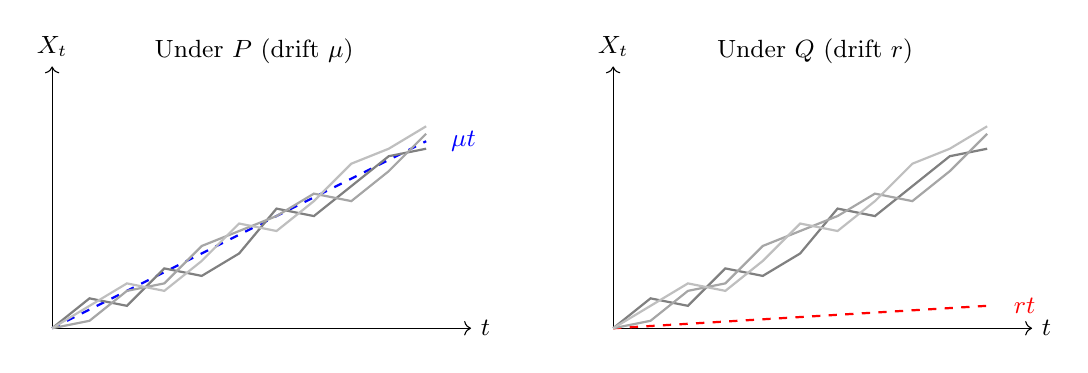
\begin{tikzpicture}[scale=0.95]
\begin{scope}[shift={(0,0)}]
\draw[->] (0,-0.3) -- (5.6,-0.3) node[right] {\small$t$};
\draw[->] (0,-0.3) -- (0,3.2) node[above] {\small$X_t$};
\node at (2.7, 3.4) {\small Under $\mathbb{P}$ (drift $\mu$)};
\draw[blue, thick, dashed] (0,-0.3) -- (5, 2.2);
\node[blue] at (5.5, 2.2) {\small $\mu t$};
\draw[gray, thick] plot coordinates {(0,-0.3)(0.5,0.1)(1,0)(1.5,0.5)(2,0.4)(2.5,0.7)(3,1.3)(3.5,1.2)(4,1.6)(4.5,2.0)(5,2.1)};
\draw[gray!70, thick] plot coordinates {(0,-0.3)(0.5,-0.2)(1,0.2)(1.5,0.3)(2,0.8)(2.5,1.0)(3,1.2)(3.5,1.5)(4,1.4)(4.5,1.8)(5,2.3)};
\draw[gray!50, thick] plot coordinates {(0,-0.3)(0.5,0)(1,0.3)(1.5,0.2)(2,0.6)(2.5,1.1)(3,1.0)(3.5,1.4)(4,1.9)(4.5,2.1)(5,2.4)};
\end{scope}

\begin{scope}[shift={(7.5,0)}]
\draw[->] (0,-0.3) -- (5.6,-0.3) node[right] {\small$t$};
\draw[->] (0,-0.3) -- (0,3.2) node[above] {\small$X_t$};
\node at (2.7, 3.4) {\small Under $\mathbb{Q}$ (drift $r$)};
\draw[red, thick, dashed] (0,-0.3) -- (5, 0);
\node[red] at (5.5, 0) {\small $rt$};
\draw[gray, thick] plot coordinates {(0,-0.3)(0.5,0.1)(1,0)(1.5,0.5)(2,0.4)(2.5,0.7)(3,1.3)(3.5,1.2)(4,1.6)(4.5,2.0)(5,2.1)};
\draw[gray!70, thick] plot coordinates {(0,-0.3)(0.5,-0.2)(1,0.2)(1.5,0.3)(2,0.8)(2.5,1.0)(3,1.2)(3.5,1.5)(4,1.4)(4.5,1.8)(5,2.3)};
\draw[gray!50, thick] plot coordinates {(0,-0.3)(0.5,0)(1,0.3)(1.5,0.2)(2,0.6)(2.5,1.1)(3,1.0)(3.5,1.4)(4,1.9)(4.5,2.1)(5,2.4)};
\end{scope}
\end{tikzpicture}
\caption{Girsanov in pictures. The two panels show the \emph{same} three sample paths. What changes is the probability weighting: under $\mathbb{P}$ these paths look typical (clustering around the trend line $\mu t$); under $\mathbb{Q}$ the same paths look like atypical upward excursions (the trend line is now the much shallower $rt$). The pathwise diffusion is identical --- only the location of the ``expected trend'' shifts. Hence the diffusion coefficient $b$ is a measure-theoretic invariant, while the drift is not.}
\label{fig:girsanov}
\end{figure}

The interpretation is striking. Under $\mathbb{P}$, the SDE
\[
  \mathrm{d}X_t=a(X_t)\,\mathrm{d}t+b(X_t)\,\mathrm{d}B_t
\]
has drift $a(X_t)$. Choose $\theta_t$ so that $b(X_t)\theta_t=\tilde a(X_t)-a(X_t)$ for a target drift $\tilde a$. Then under $\mathbb{Q}$,
\[
  \mathrm{d}X_t=a(X_t)\,\mathrm{d}t+b(X_t)(\mathrm{d}\widetilde{B}_t+\theta_t\,\mathrm{d}t)=\tilde a(X_t)\,\mathrm{d}t+b(X_t)\,\mathrm{d}\widetilde{B}_t.
\]
The diffusion coefficient is invariant under the change of measure, only the drift moves. This is a strong statement: it says the ``law of the diffusion coefficient'' (in the sense of the quadratic variation $[X]_t=\int_0^t b^2(X_s)\,\mathrm{d}s$) is a measure-theoretic invariant, while the drift can be tuned by reweighting paths.

\subsection{Application: Risk-Neutral Pricing}

In the Black--Scholes model under the real-world measure $\mathbb{P}$, the stock satisfies $\mathrm{d}S_t=\mu S_t\,\mathrm{d}t+\sigma S_t\,\mathrm{d}B_t$. The drift $\mu$ reflects the actual expected return, which is generally different from the risk-free rate $r$. Choose
\[
  \theta=\frac{r-\mu}{\sigma}
\]
(the \textbf{market price of risk}). Under the corresponding $\mathbb{Q}$,
\[
  \mathrm{d}S_t=rS_t\,\mathrm{d}t+\sigma S_t\,\mathrm{d}\widetilde{B}_t.
\]
This is the \textbf{risk-neutral} dynamics, and option prices are computed as discounted expectations under $\mathbb{Q}$ rather than $\mathbb{P}$. The mathematical content is that the same stochastic process, the same set of paths, carries two perfectly valid probabilistic interpretations; the choice of measure depends on the financial question being asked.

\section{Coda: The Big Picture}

Stepping back, the SDE--PDE bridge developed in this article forms a diagram:

\begin{figure}
    \centering
    
\includegraphics[width=0.9\linewidth]{III/fig5_bridge.png}
    \caption{Caption}
    \label{fig:placeholder}
\end{figure}

Existence/uniqueness tells us the SDE is well-posed; the Markov property says its solution carries no memory beyond its current state; the generator distills the SDE to a single linear operator; the two Kolmogorov equations translate that operator into PDEs for observables and densities; Feynman--Kac provides stochastic solutions to a wider class of parabolic equations; Girsanov tells us that drift is malleable while diffusion is not.

In the next installment we will use this machinery to study \textbf{specific} families of SDEs: linear SDEs, the CIR process, and the Heston stochastic volatility model, and develop tools (the change of variables, time changes, the Lamperti transform) that turn nonlinear SDEs into tractable ones.

\appendix

\section{Gronwall's Inequality\label{app:gronwall}}

The proofs in this article (and in [II]) all reduce to controlling a function $\phi(t)\ge 0$ that satisfies an integral inequality of the form
\[
  \phi(t)\le \alpha+\beta\!\int_0^t\phi(s)\,\mathrm{d}s.
\]
\textbf{Gronwall's lemma} (integral form) states that any such $\phi$, when $\alpha,\beta\ge 0$ are constants, satisfies
\[
  \phi(t)\le \alpha\,e^{\beta t}.
\]
The proof is two lines: let $\Phi(t)=\alpha+\beta\!\int_0^t\phi$, then $\Phi'=\beta\phi\le\beta\Phi$, so $(\Phi e^{-\beta t})'\le 0$, giving $\Phi(t)\le\Phi(0)e^{\beta t}=\alpha e^{\beta t}$, and $\phi\le\Phi$ closes the argument.

For SDE applications one often needs a slightly more general version where $\alpha$ is a non-decreasing function of $t$: if $\phi(t)\le\alpha(t)+\beta\!\int_0^t\phi(s)\,\mathrm{d}s$, then $\phi(t)\le\alpha(t)e^{\beta t}$. The proof is identical.

\section{Details of the Existence/Uniqueness Theorem\label{app:exuniq}}

We sketch the bookkeeping for Step 2 of the Picard iteration. Define the difference $D^{(n)}_t=X^{(n+1)}_t-X^{(n)}_t$. Then
\[
  D^{(n)}_t=\int_0^t\!\bigl[a(s,X^{(n)}_s)-a(s,X^{(n-1)}_s)\bigr]\mathrm{d}s+\int_0^t\!\bigl[b(s,X^{(n)}_s)-b(s,X^{(n-1)}_s)\bigr]\mathrm{d}B_s.
\]
Apply the elementary inequality $(p+q)^2\le 2p^2+2q^2$, take the supremum over $s\le t$ inside the expectation, and use \textbf{Doob's $L^2$ inequality} on the martingale piece:
\[
  \mathbb{E}\sup_{s\le t}\!\left|\int_0^s\![b(r,X^{(n)}_r)-b(r,X^{(n-1)}_r)]\mathrm{d}B_r\right|^2\le 4\mathbb{E}\!\int_0^t\!|b(r,X^{(n)}_r)-b(r,X^{(n-1)}_r)|^2\mathrm{d}r.
\]
For the drift piece, Cauchy--Schwarz gives a similar bound with a $t$ in front. Using the Lipschitz condition (L),
\[
  \mathbb{E}\sup_{s\le t}|D^{(n)}_s|^2\le K_1\!\int_0^t\mathbb{E}\sup_{r\le s}|D^{(n-1)}_r|^2\,\mathrm{d}s,
\]
where $K_1=2L^2(t+4)$ can be bounded uniformly by $K_1=2L^2(T+4)$ on $[0,T]$. Iterating $n$ times yields
\[
  \mathbb{E}\sup_{s\le T}|D^{(n)}_s|^2\le \frac{(K_1 T)^n}{n!}\,\mathbb{E}\sup_{s\le T}|D^{(0)}_s|^2,
\]
and the factorial denominator wins against the exponential numerator, giving summability.

Step 3 (uniqueness) is the same computation with $D=X-Y$ for two purported solutions: one finds $\mathbb{E}\sup_{s\le t}|D_s|^2\le K_1\!\int_0^t\mathbb{E}\sup_{r\le s}|D_r|^2\,\mathrm{d}s$, and Gronwall (with $\alpha=0$) closes the loop.

\section{Quick Reference: Operators and Their Adjoints\label{app:adjoint}}

For the operator $\mathcal{L}=a(x)\partial_x+\tfrac{1}{2}b^2(x)\partial_{xx}^2$ acting on smooth functions, integration by parts twice yields the formal adjoint
\[
  \mathcal{L}^*\rho=-\partial_x(a\rho)+\tfrac{1}{2}\partial_{xx}^2(b^2\rho),
\]
satisfying $\int(\mathcal{L}u)\rho\,\mathrm{d}x=\int u(\mathcal{L}^*\rho)\,\mathrm{d}x$ whenever boundary terms vanish. The asymmetry $a$ remains inside a single derivative while $b^2$ sits under two, reflects the different parities of the drift and diffusion contributions and is essentially the same fact, viewed from a different angle, as why the generator has $a\partial_x$ (first order) and $\tfrac{1}{2}b^2\partial_{xx}^2$ (second order).

In multivariate form ($X_t\in\mathbb{R}^d$, $a:\mathbb{R}^d\to\mathbb{R}^d$, $b:\mathbb{R}^d\to\mathbb{R}^{d\times m}$, $\sigma=bb^\top$),
\[
  \mathcal{L}=\sum_i a_i\,\partial_i+\tfrac{1}{2}\sum_{i,j}\sigma_{ij}\,\partial_{ij}^2,\qquad
  \mathcal{L}^*\rho=-\sum_i\partial_i(a_i\rho)+\tfrac{1}{2}\sum_{i,j}\partial_{ij}^2(\sigma_{ij}\rho).
\]
All of the theorems in this article extend mutatis mutandis to the multivariate case; the proofs are notationally heavier but conceptually identical.

\end{CJK*}
\end{document}
